\documentclass[scrartcl]{article}
\usepackage[sexy]{evan}
% \usepackage{geometry}
% \geometry{total={170mm,250mm}, top=25mm}

\usepackage{graphicx} % Required for inserting images
\usepackage{amsmath}
\date{}
\author{}
\usepackage[utf8]{inputenc}
\usepackage{fancyhdr}
\usepackage{algorithm}
\usepackage{listings}
\usepackage{algpseudocode}
% Default fixed font does not support bold face
\DeclareFixedFont{\ttb}{T1}{txtt}{bx}{n}{8} % for bold
\DeclareFixedFont{\ttm}{T1}{txtt}{m}{n}{8}  % for normal

% Custom colors
\usepackage{color}
\definecolor{deepblue}{rgb}{0,0,0.5}
\definecolor{deepred}{rgb}{0.6,0,0}
\definecolor{deepgreen}{rgb}{0,0.5,0}

\usepackage{listings}

% Python style for highlighting
\newcommand\pythonstyle{\lstset{
language=Python,
basicstyle=\ttm,
morekeywords={self},              % Add keywords here
keywordstyle=\ttb\color{deepblue},
emph={MyClass,__init__},          % Custom highlighting
emphstyle=\ttb\color{deepred},    % Custom highlighting style
stringstyle=\color{deepgreen},
frame=tb,                         % Any extra options here
showstringspaces=false
}}


% Python environment
\lstnewenvironment{python}[1][]
{
\pythonstyle
\lstset{#1}
}
{}
\title{Universal Source Coding: Explorations in Information Theory and Encoding Schemes}
\usepackage[toc,page]{appendix}
\DeclareMathOperator*{\Index}{\textbf{Index}}
\fancyhf{}
\fancyhead[L]{Bachelors of Statistics (Hons.), 2023-26}
\fancyfoot[C]{\thepage}
\setlength{\headsep}{35pt}
\renewcommand{\footrule}{
        \hrule width\headwidth height\headrulewidth depth\headrulewidth
}

\usepackage{enumitem}
\begin{document}
\begin{titlepage}
\newcommand{\HRule}{\rule{\linewidth}{0.5mm}} % Defines a new command for the horizontal lines, change thickness here

%----------------------------------------------------------------------------------------
%	LOGO SECTION
%----------------------------------------------------------------------------------------
\centering

\includegraphics[width=6cm]{title/logo.png}\\[1cm] % Include a department/university logo - this will require the graphicx package
 
%----------------------------------------------------------------------------------------

\center % Center everything on the page

%----------------------------------------------------------------------------------------
%	HEADING SECTIONS
%----------------------------------------------------------------------------------------

\textsc{\LARGE \assignname}\\[1.5cm] %assignment name
\textsc{\Large \coursecode}\\[0.5cm] %Course code 
\textsc{\large \coursetitle}\\[0.5cm]  %Course title

%----------------------------------------------------------------------------------------
%	TITLE SECTION
%----------------------------------------------------------------------------------------
\makeatletter
\HRule \\[0.4cm]
{ \huge \bfseries \@title}\\[0.1cm] % Title of your document
\HRule \\[1.5cm]
 
%----------------------------------------------------------------------------------------
%	AUTHOR SECTION
%----------------------------------------------------------------------------------------


\begin{minipage}{0.4\textwidth}
\begin{flushleft} 
Himadri Mandal (BS2327)\\
Siddhartha Bhattacharya (BS2345)
\end{flushleft}
\end{minipage}
\begin{minipage}{0.4\textwidth}
\begin{flushright} 
Abhik Rana (BS2301)\\
Ayan Ghosh (BS2321)
\end{flushright}
\end{minipage}\\[2cm]
\makeatother

\textit{\large Advisor/Instructor}\\
\Large \textbf{DR. ARNAB CHAKRABORTY} \\
Associate Professor, Applied Statistics Unit\\[2cm]


{\large Monday $\text{27}^{\text{th}}$ November, 2023}\\[2cm]
\vfill

\end{titlepage}
\pagestyle{fancy}
\maketitle
\author{}
\date{}
\begin{abstract}
    Morse code sends English characters using dots and dashes. The letter E is represented by a single dot. This is reasonable because E happens to the most frequently occuring letter in normal usage. So assigning the shortest code to it makes sense from the viewpoint of length optimisation. 
    The intuitive idea of ``more frequent inputs should be mapped to shorter outputs" gets rigorised in the so-called Huffman encoding scheme. It turns out to be the optimal encoding scheme given you know the source distribution. This project tries to answer the natural extension to that question: to come up with an encoding scheme that guarantees a minimum performace against all input probability distributions, \textit{algorithmically.}
\end{abstract}
\section{Introduction}
The broad setup is the following: there's data coming in from some source. If the source distribution is known, then Huffman Encoding gives the optimal encoding scheme. This project tries to figure out a good encoding scheme (in multiple contexts!) that guarantees performance against all source distributions!
There are many ways to go about this project, and we thought it would be a very big missed opportunity if we just explore one of them, so we decided to pursue our creativity and explore the multiple perspectives we found out!

Himadri Mandal and Abhik Rana have improved the \textbf{Lempel-Ziv-Welch} algorithm in a particular context, Ayan Ghosh used \textbf{Method of Types} to prove that the Naive Idea doesn't work, and he showed an extension of a result, as we see. Siddhartha Bhattacharya has worked on a \textbf{Huffman Encoding focused approach}. 

There were a few other approaches that we also worked on but those weren't particularly promising. First, we would like to go through the transition of ideas we went through. 

\section {Initial Ponderings}
\begin{context}
Data comes in character by character. We don't know the source distribution of the data. Therefore, we try to estimate the source distribution and use the many techniques available thereon.
\end{context}

\subsection{Naive Idea \#1: Estimate using the Empirical CDF}
We can wait till the $n^{\text{th}}$ character is inputted and use that to find the empirical CDF $\hat{P}$
and then use Huffman Encoding on it. But, this is a terrible idea and we prove why:
\begin{theorem*}
Huffman Encoding a truncated input stream based on its Empirical Distribution $\hat{P}$ is \textit{not} a Universal Source Code. 
\end{theorem*}
\begin{proof}
Let $\Omega$ be the character set. Let $I$ be the truncated input stream of length $k$. Create a set $A$ consisting of the Huffman encoded words based on this truncated input stream and its empirical probability distribution $\hat{P}$

Mathematically the encoder is \[
f_n(x) = \begin{cases} 
 \text{Huffman encoding of x} & x \in A \\
 0 & x \notin A
 \end{cases}
\]

The decoder is the Huffman decoder. 
Now in this setup, we calculate the probability of error. Assuming that the code $X_1, X_2, \cdots X_m$ are coming from an arbitrary distribution Q. Denote the probability of a subset C of $\Omega^n$ coming from the distribution Q as $Q^n(C) $. 

$$P_e^{(n)} = 1- Q^n(A) \geq 1 - 2^{-nD_{KL}(\hat{P}||Q)}$$
$$D_{KL}(\hat{P} || Q) = \sum\limits_{\omega} \hat{P}(\omega) log\left(\frac{\hat{P}(\omega)}{Q(\omega)}\right)$$ which is independent of n. 

Therefore $P_e^{(n)} \rightarrow 1$ as $n \rightarrow \infty$.
\end{proof}
\subsection{Idea \#2:}
If you know the source distribution already, then you're done. What we can do is try to define a ``universe" of distributions and figure out a good ``center" of this universe. By universe I mean a probability simplex: 

\begin{proposition*}
    Let $\{p_1, p_2, \cdots, p_m\}$ be a set of pmfs. Define the universe of probabilities to be
    $$\mathcal{U} = \Bigg\{\alpha_1 \cdot p_1 + \cdots + \alpha_m \cdot p_m \Bigg| \alpha_1 + \cdots + \alpha_m = 1, 0 \leq \alpha_i \leq 1\Bigg\}$$
\end{proposition*}
\begin{proposition*}
    Let $\chi_d(P,Q)$ be a measure of ``difference'' between two probability distributions $P, Q$. Let $\mathcal{U}$ be a universe of probabilities. Define the two following centers of universe: $\mathcal{P}_{1}$ and $\mathcal{P}_{2}$
    $$\mathcal{P}_1 = \underset{P}{\arg \min} \underset{Q \ \sim \ \mathcal{U}}{\Bbb{E}}[\chi_d(P,Q)]$$
    $$\mathcal{P}_2 = \underset{P \ \sim \ U}{\inf} \underset{Q \ \sim \ U}{\sup} \ \chi_d(P,Q)$$
    $\mathcal{P}_1, \mathcal{P}_2$ give best average performace and best worst performance, respectively.
\end{proposition*}

The measure of difference between two probability distribution we tried to work with was $\chi_d(P,Q) = \operatorname{D_{KL}}(Q || P)$.
The idea is the following:
\begin{itemize}
    \item Figure out a good way to fix the universe $\mathcal{U}$. 
    \item Find the centers $\mathcal{P}_!$, $\mathcal{P}_2$ using gradient descemt or such.
    \item Obtain encoding schemes $H_1, H_2$ accordingly. Choose as need be. 
\end{itemize}
We believe there is promise in this idea, and should be explored further. However, we figured out new perspectives to look at this problem and so didn't devote any more time into this.
\subsection{An extension of a result}
\begin{theorem*}
For any $R>0$, an increasing sequence $R_n \uparrow R$, determines a universal source code of length n having size $O(2^{nR})$.
\end{theorem*}

\begin{proof}
Fix $R>0$ . For each sequence $x \in \Omega^n$, denote its empirical distribution by $P(x)$. Denote a sequence $y \in P(x)$ if it has same distribution as that of $x$. Denote the cardinality of such a set as $T(P(x))$
Denote the set $A = \{ x \in \Omega^n : H(P(x))\leq R_n\}$. 

$|A|= \sum\limits_{y: y \in P(x), x \in A} 1 = \sum\limits_{x \in A} T(P(x)) \leq  \sum\limits_{x \in A} 2^{nH(P(x))} \leq 2^{nR_n} (n+1)^{|\Omega|} $ which gives $|A| = O(2^{nR})$ 

Now to show this scheme is universal. Define the encoder 
\[
f_n(x) = \begin{cases} 
 \text{index of x in A} & x \in A \\
 0 & x \notin A
 \end{cases}
\]

The decoder maps the index back to A. The underlying distribution is Q where $H(Q)<R$.  

Therefore $P_e^{(n)} = 1- Q^n(A) = \sum\limits_{P:H(P)>R_n}Q^n(T(P)) \leq (n+1)^{|\Omega|} \max\limits_{P:H(P)>R_n} Q^n(T(P))$. 
Now we use the bound $Q^n(T(P)) \leq 2^{-nD(P||Q)}$ 
to get $P_e^{(n)}\leq (n+1)^{|\Omega|} 2^{ -n \min\limits_{P: H(P)>R_n} D(P||Q)}$.

Since $R_n \uparrow R$, we can say that for some $N$, $\forall n\geq N $, $H(Q)\leq R_n$. 

This gives $ H(P_n) = H(\arg \max_{P:H(P)>R_n} Q^n(T(P))) >H(Q) $.  

Hence by Gibbs inequality, $\min\limits_{P: H(P)>R_n} D(P||Q) >$ for all $n>N$. 
Therefore $P_e^{(n)} \rightarrow 0$, completing the proof. 
\end{proof}

\section{Bubbly Lempel-Ziv-Welch}
\subsection{Theory}
We improve the \textbf{Lempel-Ziv-Welch} algorithm. We named this ``\text{Bubbly}'' because the initial versions of our work somehow represented the bubble sort. 

\begin{context}
    $\textbf{Lossless File Compression}$. We have a file $F$ with letters $\text{(a-z)}$. We compress the file $F$ and create $E(F)$ in a way that if the $\textbf{Decoder}$ has the knowledge of $E(F)$ and the encoding scheme $E(\cdot)$ then it can rediscover $F$ with no loss. Ofcourse we care about time and space complexities. 
\end{context}
\begin{proposition*}[Lempel-Ziv-Welch]
    Define dictionary $D$ with all characters in the input alphabet and their encodings. Define a running string variable $\operatorname{Pattern}$, and iteratively add the next character to it. If the resulting string is already in $D$, continue reading characters until you find a string that is \textit{not} in the dictionary $D$. Add it to $D$ with its encoding. Then, encode $\operatorname{Pattern}$ as $D[\operatorname{Pattern}[0:-1]] + \operatorname{Pattern}[-1]$. Continue.
\end{proposition*}
\begin{example*}
    \text{Text = AABABBABBAABABBA}
    \newline
    \text{Dictionary: A - 1, AB - 2, ABB - 3, ABBA - 4, ABA - 5, B - 6, BA - 7}
    \newline
    \text{Encoded = A1B2B3A2A\#B6A}

\end{example*}
Canonically, the encodings of $D$ follow a monotonic ordering in the time axis. This is to prevent what we call ``ambiguities'' as we see.
To improve this algorithm: we attack the way encodings are determined. Clearly, in the attempt to make the algorithm simple and the decoding direct $\textbf{LZW}$ makes no effort in determining optimal encodings.
To do this, we need two things: 
\begin{itemize}
    \item For any permutation $\xi(D)$ of the encodings, we should be able to perform the decoding scheme $\textit{without}$ a lookup table!
    \item Optimize $\xi(D)$ for length of text. 
\end{itemize}
The second part is easier to ensure, so let's do that first.

\begin{proposition*}[\textbf{Bubbly LZW: Permutation optimization}]
    Obtain the normal $\textbf{LZW}$ dictionary $D$, and find the number of times each encoding is obtained, for a phrase $X$
    call this $\operatorname{Counter}(X)$. Sort $D$ in decreasing order according to the key $f(v) = \operatorname{len}(v)\cdot\operatorname{Counter}(v)$. \newline

    Define $P_D = \operatorname{SortedD}^{-1}$ such that $\operatorname{SortedD}[P_D(x)] = x$. $P_D$ is the optimized permutation.
\end{proposition*}

Okay, let's try to figure out the first obstacle now. 
\begin{definition*}[Phrase]
    Phrases are of three types:
    \begin{enumerate}
        \item Parent: $\text{(}n\text{X)}$, where $n$ is an encoding whose definition can not be realized given the text before this phrase and $\text{X}$ is some character.
        \item Child: $\text{(}n\text{X)}$, where $n$ is an encoding whose definition can be realized using the text before this phrase and $\text{X}$ is some character.
        \item New: $\text{(\#X)}$, where $\text{X}$ is some character.
    \end{enumerate}
\end{definition*}
\begin{proposition*}[Phrase Decomposition]
    Let $\xi(D)$ be a permutation of the encoding. Using this permutation of the encoding, encode the text. Obtain $E_{\xi}(\text{Data})$. Define 
    $\textbf{Phrase Decomposition}$ of $E_{\xi}(\text{Data})$ to be a decomposition of the encoded text into phrases.
\end{proposition*}
\begin{example*}
    \text{Text = \#a3b1b2a1a\#b4a}
    \newline
    \text{Phrase Decomposition = (\#a)(3b)(1b)(2a)(1a)(\#b)(4a)}
\end{example*}
As the decoder reads through the encoded, there could arise what we call "ambiguities". An example of such a thing is:
\begin{example*}[Ambiguity]
    \text{Phrase Decomposition = (\#a)(3b)(1b)(2a)(1a)(\#b)(4a)}
    \newline
    Here ``(1a)'' is an ambiguous phrase whose meaning cannot be derived by the decoder using the phrases before it. 
\end{example*}
When we obtain ambiguities it is necessary for us to define it out for the decoder to then use it. Here is a characterisation of ambiguities:
\begin{theorem*}[Characterisation of The First Ambiguity]
    A phrase $P$ is the first ambiguity $\iff$ the phrase $P$ is the last parent phrase before the first child phrase (OR) the last parent phrase before the first new phrase. 
\end{theorem*}
This leads us to the algorithm of finding out the ambiguities and then solving them:
\algdef{SE}[SUBALG]{Indent}{EndIndent}{}{\algorithmicend\ }%
\algtext*{Indent}
\algtext*{EndIndent}
\begin{algorithm}
    \caption{ Recursively solve ambiguities. }\label{riffle}
    \begin{algorithmic}[1]
    \Procedure{SolveAmbiguity}{Encoded}
        \While{IsAmbiguity: \textbf{True}}
        \State Find the \textbf{first occurence} of one of the two:
        \Indent
            \State \textbf{(parent)(child)}
            \State \textbf{(parent)(new)}
        \EndIndent

        \State Perform the \textit{definition} of the \textbf{(parent)}
        \State Mark the next phrase a parent, and continue.
        \EndWhile
    \EndProcedure
    \end{algorithmic}
\end{algorithm}
\begin{proposition*}[Defining a Parent]
    By defining a parent phrase $P$, we mean giving the decoder some information that can then be used to determine the encoding 
    of $P$ unambiguously. Here we used the most naive idea: we defined a parent phrase $P$ by attaching its definition to it.
\end{proposition*}
\newpage
Albeit a bit complicated, here's the decoder algorithm:
\begin{python}
    class Decoding:
        def __init__(self, unambiguous):
            self.code = unambiguous 
        
        def nearest_closing_bracket(self, idx):
            j = 1
            while self.code[idx+j] != ')':
                j+=1
            return idx+j, self.code[idx+1:idx+j]
        
        def farthest_ending_digit(self, idx):
            j = 0
            while self.code[idx+j].isnumeric():
                j += 1
            return idx+j-1, self.code[idx:idx+j]
        
        def return_key(self, dictionary, idx):
            return list(dictionary.keys())[list(dictionary.values()).index(idx)]
        
        def decoder(self):
        dictionary = {}
            decode = ''
            i = 0
            while i < len(self.code):
                if self.code[i] == '#':
                    if self.code[i+2] == '(': 
                        ending_bracket, inside = self.nearest_closing_bracket(i+2)
                        dictionary[self.code[i+1]] = int(inside)
                        i = 1+ending_bracket
                        decode += self.code[i+1]
                    else:
                        ending_location, address = self.farthest_ending_digit(i+2)
                        dictionary[self.code[i+1]] = int(address)
                        i = 1 + ending_location
                        decode += self.code[i+1]
                else:
                    j, prev = self.farthest_ending_digit(i)
                    if self.code[j+2] == '(':
                        ending_bracket, inside = self.nearest_closing_bracket(j+2)
                        dictionary[self.return_key(dictionary, int(prev))+self.code[j+1]] = int(inside)
                        decode += self.return_key(dictionary, int(prev))+self.code[j+1]
                        i = 1+ending_bracket
                    else:
                        ending_location, address = self.farthest_ending_digit(j+2)
                        dictionary[self.return_key(dictionary, int(prev))+self.code[j+1]] = int(address)
                        decode += self.return_key(dictionary, int(prev))+self.code[j+1]
                        i = 1 + ending_location
            print(dictionary)
            return decode    
\end{python}
\subsection{Results and Observations}
We plot the improvements achieved by $\textbf{BLZW}$ over $\textbf{LZW}$ in the following graph:
\begin{figure}[H]
    \centering
    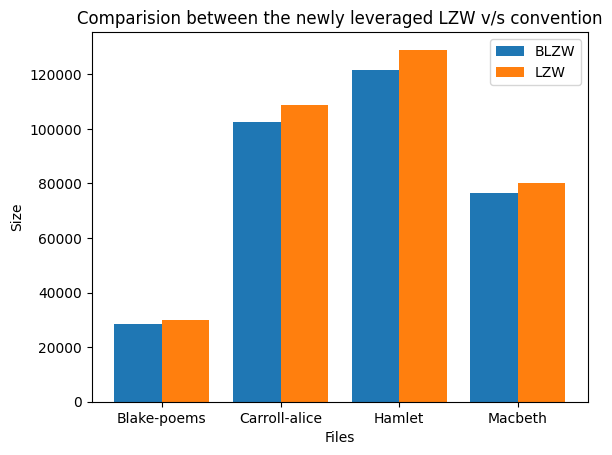
\includegraphics[width=0.7\textwidth]{blzwvslzw.png}
    \caption{Improvement on Language Datasets}
    \label{fig:example}
\end{figure}
\section{Huffman Must Encode}
\subsection{Huffman Encoding}
Formalized description 

\textbf{Input.}
Alphabet $A=\left(a_1, a_2, \ldots, a_n\right)$, which is the symbol alphabet of size $n$.
Tuple $W=\left(w_1, w_2, \ldots, w_n\right)$, which is the tuple of the (positive) symbol weights (usually proportional to probabilities), i.e. $w_i=\operatorname{weight}\left(a_i\right), i \in\{1,2, \ldots, n\}$.

\textbf{Output.}
Code $C(W)=\left(c_1, c_2, \ldots, c_n\right)$, which is the tuple of (binary) codewords, where $c_i$ is the codeword for $a_i, i \in\{1,2, \ldots, n\}$

\textbf{Goal.}
Let $L(C(W))=\sum_{i=1}^n w_i$ length $\left(c_i\right)$ be the weighted path length of code $C$. Condition: $L(C(W)) \leq L(T(W))$ for any code $T(W)$.

\subsection{Proof of Optimality}
Recall that the problem is given frequencies $f_1, \ldots, f_n$ to find the optimal prefix-free code that minimizes
$$
\sum_i^n f_i \cdot \text { length of encoding of the } i \text {-th symbol. }
$$

This is the same as finding the full binary tree with $n$ leaves, one per symbol in $1, \ldots, n$, that minimizes
$$
\sum_{i=1}^n f_i \cdot(\text { depth of leaf of the } i \text {-th} symbol) 
$$


\begin{claim}[Huffman's Claim]
    There's an optimal tree where the two smallest frequency symbols mark siblings (which are at the deepest level in the tree).
\end{claim}
\begin{claim}
    Huffman's coding gives an optimal cost prefix-tree tree.
\end{claim}
Proof. The proof is by induction on $n$, the number of symbols. The base case $n=2$ is trivial since there's only one full binary tree with 2 leaves.

Inductive Step: We will assume the claim to be true for any sequence of $n-1$ frequencies and prove that it holds for any $n$ frequencies. Let $f_1, \ldots, f_n$ be any $n$ frequencies. Assume without loss of generality that $f_1 \leq f_2 \leq \ldots \leq f_n$ (by relabeling). By Claim 1, there's an optimal tree $T$ for which the leaves marked with 1 and 2 are siblings. Let's denote the tree that Huffman strategy gives by $H$. Note that we are not claiming that $T=H$ but rather that $T$ and $H$ have the same cost.

We will now remove both leaves marked by 1 and 2 from $T$, making their father a new leaf with frequency $f_1+f_2$. This gives us a new binary tree $T^{\prime}$ on $n-1$ leaves with frequencies $f_1+f_2, f_3, f_4, \ldots, f_n$. We do the same for the Huffman tree giving us a tree $H^{\prime}$ on $n-1$ leaves with frequencies $f_1+f_2, f_3, f_4, \ldots, f_n$. Note that $H^{\prime}$ is exactly the Huffman tree on frequencies $f_1+f_2, f_3, f_4, \ldots, f_n$ by definition of Huffman's strategy. By the induction hypothesis,
$$
\operatorname{cost}\left(H^{\prime}\right)=\operatorname{cost}\left(T^{\prime}\right) .
$$

Observe further that
$$
\operatorname{cost}\left(T^{\prime}\right)=\operatorname{cost}(T)-\left(f_1+f_2\right)
$$
since to get $T^{\prime}$ from $T$ we replaced two nodes with frequencies $f_1$ and $f_2$ at some depth $d$ with one node with frequency $f_1+f_2$ at depth $d-1$. This lowers the cast by $f_1+f_2$. Similarly,
$$
\operatorname{cost}\left(H^{\prime}\right)=\operatorname{cost}(H)-\left(f_1+f_2\right) .
$$

Combining the three equations together we have that
$$
\operatorname{cost}(H)=\operatorname{cost}\left(H^{\prime}\right)+f_1+f_2=\operatorname{cost}\left(T^{\prime}\right)+f_1+f_2=\operatorname{cost}(T) .
$$

\subsection{Variant-Adaptive Huffman Coding}
 
In consideration of a variable character distribution, we engage with data processing tasks wherein data arrives in sequential chunks. Our objective is to encode each incoming chunk efficiently while simultaneously maintaining a dictionary structure to facilitate straightforward decoding operations. This process is fundamental for tasks such as data compression, where the adaptability of encoding schemes to fluctuating character frequencies is paramount.

To achieve this, we implement an Adaptive Huffman coding algorithm. This algorithm dynamically adjusts its encoding tree structure as new symbols are encountered, ensuring adaptability to evolving character distributions. The essence of our approach lies in the concurrent encoding of incoming data chunks and the maintenance of a dictionary that correlates encoded symbols to their respective characters. This dictionary plays a crucial role in the decoding process, enabling the reconstruction of the original data from its encoded representation.

Formally, our Adaptive Huffman coding implementation comprises the following components:

1. \textbf{Data Encoding}:
   - As each chunk of data arrives, we encode it using the Adaptive Huffman algorithm. This involves traversing the encoding tree to generate binary representations of the input symbols.

2. \textbf{Dictionary Maintenance}:
   - Simultaneously, we update and maintain a dictionary that maps each symbol to its corresponding binary code. This dictionary serves as a reference for decoding operations and evolves dynamically alongside the encoding process.

3. \textbf{Dynamic Tree Adjustment}:
   - The Adaptive Huffman algorithm dynamically adjusts the encoding tree structure based on the frequency of encountered symbols. This adaptability ensures optimal encoding efficiency, with more frequently occurring symbols assigned shorter binary codes.

4. \textbf{Decoding Process}:
   - To decode encoded data, we utilize the maintained dictionary to efficiently map binary codes back to their original symbols. The dynamic nature of the encoding tree ensures that decoding operations remain efficient and accurate across varying character distributions.

By formalizing these components, we establish a robust framework for encoding and decoding sequential data chunks while accommodating diverse character distributions. This approach ensures efficient data compression and facilitates seamless communication and storage of information in real-world applications.
\subsection{Combining the Above}
To implement the following algorithm effectively, it's crucial to understand its key components and the sequential flow of operations. Here's a formal description of the algorithm:

1. \textbf{Dictionary Concatenation}:
   - When a user writes another piece of text, the same process is repeated to obtain optimal weights and create a corresponding dictionary.
   - If the ordering of weights remains the same, indicating no significant changes in the character frequencies, the new dictionary is concatenated with the previous one.
   - If the ordering of weights changes, suggesting a shift in character frequencies, the differences in the encoding scheme are noted and incorporated into the dictionary.

2. \textbf{Initialization}:
   - Given an initial encoding scheme \( E_1 \), weight vector \( W_1 \), and dictionary \( D_1 \), encode the first chunk of text using \( E_1 \) and maintain \( D_1 \).

3. \textbf{Updating Encoding Scheme}:
   - Upon adding a new chunk of text with weight vector \( W_2 \), construct a new dictionary \( D_2 \) corresponding to the new text.
   - Check the monotonicity of \( W_2 \) and \( W_1 + W_2 \):
     - If the monotonicity of \( W_2 \) matches \( W_1 + W_2 \), continue using \( E_1 \).
     - If the monotonicity of \( W_2 \) differs from \( W_1 + W_2 \):
       - Determine the smallest number of permutations required for \( W_2 \) to achieve the same monotonicity as \( W_1 + W_2 \).
       - Update \( D_1 \) accordingly by applying the permutations, ensuring that the changes preserve existing encodings as much as possible.
       - Use the modified dictionary \( D_1 \) to encode the new chunk of text with \( E_1 \).

4. \textbf{Recursion and Separate Computation}:
   - Repeat the above process recursively for subsequent chunks of text.
   - If the set of indexes of non-zero weights of \( W_2 \) is a subset or equal set of indexes of non-zero weights of \( W_1 \):
     - Check if the monotonicity of \( W_1 + W_2 \) and \( W_2 \) is preserved.
     - If preserved, continue with \( E_1 \); otherwise, update \( D_1 \) and \( E_1 \) as described above.
   - If none of the indexes of non-zero weights of \( W_2 \) is a subset or equal set of indexes of non-zero weights of \( W_1 \):
     - Compute the dictionary \( D_2 \) separately.
   - If the indexes of non-zero weights of \( W_2 \) have a non-zero intersection with the indexes of non-zero weights of \( W_1 \):
     - Again, compute the dictionary \( D_2 \) separately.

This formal description outlines the procedure for adaptively updating the encoding scheme and dictionary based on changes in the weight vectors of chunks of text. It accounts for scenarios where the monotonicity changes and where the sets of non-zero weights intersect or are disjoint between weight vectors.

Now we can recursively keep on storing the dictionary by noting the changes being made so we dont have to collectively store a complete dictionary everytime we add a new chunk of data which will make the decoding a simple recursive process
\end{document}